\documentclass[]{beamer}
\usepackage{graphicx,comment}

\let\epsilon\varepsilon
\newcommand{\Mon}{\operatorname{Mon}\;}
\newcommand{\Inv}{\operatorname{Inv}\;}
\newcommand{\pskip}{\medskip}
\newcommand{\pmat}[1]{\begin{pmatrix} #1 \end{pmatrix}}
\DeclareMathOperator{\GL}{GL}
\DeclareMathOperator{\GF}{GF}

\title{One-relation semigroups and their word problem}
\author{Lucas Jones}
\date{3rd April, 2017}
\institute{University of St Andrews}

\beamertemplatenavigationsymbolsempty
\definecolor{inactive}{RGB}{230,230,230}

\begin{document}

\maketitle

\begin{frame}{Groups, semigroups, monoids}
	A \textbf{\textcolor{inactive}{semi}group} is a set $S$ together with a binary operation $\cdot \colon S \times S \to S$ such that:

	\begin{enumerate}
		\item \emph{[Associativity]} $(a \cdot b) \cdot c = a \cdot (b \cdot c)$ for all $a, b, c \in S$
		\item \emph{[Identity]} there exists a distinguished element $\epsilon \in S$ such that $\epsilon \cdot x = x \cdot \epsilon = x$ for all $x \in S$
		\item \emph{[Inverses]} for every element $x \in S$, there exists a unique element $x^{-1} \in S$ such that $x \cdot x^{-1} = x^{-1} \cdot x = \epsilon$
	\end{enumerate}

	\note{
		So hopefully everyone here knows what a group is, you know, you have a set together with some binary operation which is associative --- we don't care where the brackets go. We have an identity element, if we multiply either side by that then we get the same thing out... and every element has an inverse. Multiply either side by that and we get the identity.
	}
\end{frame}

\begin{frame}{Groups, semigroups, monoids}
	A \textbf{semigroup} is a set $S$ together with a binary operation $\cdot \colon S \times S \to S$ such that:

	\begin{enumerate}
		\item \emph{[Associativity]} $(a \cdot b) \cdot c = a \cdot (b \cdot c)$ for all $a, b, c \in S$
		\textcolor{inactive}{
		\item \emph{[Identity]} there exists a distinguished element $\epsilon \in S$ such that $\epsilon \cdot x = x \cdot \epsilon = x$ for all $x \in S$
		\item \emph{[Inverses]} for every element $x \in S$, there exists a unique element $x^{-1} \in S$ such that $x \cdot x^{-1} = x^{-1} \cdot x = \epsilon$
			}
	\end{enumerate}

	\note{
		So from there, we generalise to semigroups --- we call them that because we got rid of half of the axioms (as we know, half of 3 is 1). Now all we have is a set with a binary operation on it: we don't necessarily have an identity or an inverse. Obviously there's not as much structure there.
	}
\end{frame}

\begin{frame}{Groups, semigroups, monoids}
	A \textbf{monoid} is a set $S$ together with a binary operation $\cdot \colon S \times S \to S$ such that:

	\begin{enumerate}
		\item \emph{[Associativity]} $(a \cdot b) \cdot c = a \cdot (b \cdot c)$ for all $a, b, c \in S$
		\item \emph{[Identity]} there exists a distinguished element $\epsilon \in S$ such that $\epsilon \cdot x = x \cdot \epsilon = x$ for all $x \in S$
		\textcolor{inactive}{
		\item \emph{[Inverses]} for every element $x \in S$, there exists a unique element $x^{-1} \in S$ such that $x \cdot x^{-1} = x^{-1} \cdot x = \epsilon$
			}
	\end{enumerate}

	\note{
		In this talk we're going to talk mostly about a structure in between --- a monoid. We give ourselves back an identity element in a semigroup.
	}
\end{frame}


\begin{frame}{Free semigroups}
	Let $A$ be a finite set.

	Then the \textbf{free semigroup} on $A$, denoted $A^+$, is the set of all words with letters in $A$, under the operation of concatenation. \phantom{, \emph{including an empty string $\epsilon$}}

	\note{
		The first class of semigroups we'll introduce are the free semigroups. We take an alphabet --- just a set of `letters', finite in our case --- and our underlying set is the set of all nonempty strings consisting of words made up of these letters. Our operation is concatenation of strings, which it's hopefully fairly clear is associative.
	}

	\pause
	\bigskip

	\begin{block}{Example}
		If $A = \{a, b\}$, then $A^+ = \{a, b, aa, ab, ba, bb, aaa, aab, \ldots\}$. \\
		Multiplying, $aa \cdot b = aab$.
	\end{block}

	\note{
		Here's an example. Let's suppose our alphabet is $\{a, b\}$. So we have all the words, finite sequences of $a$s and $b$s. To multiply them, stick them together.
	}
\end{frame}

\begin{frame}{Free monoids}
	Let $A$ be a finite set.

	Then the \textbf{free monoid} on $A$, denoted $A^*$, is the set of all words with letters in $A$, under the operation of concatenation, \emph{including an empty string $\epsilon$}.

	\bigskip

	\begin{block}{Example}
		If $A = \{a, b\}$, then $A^* = \{\epsilon, a, b, aa, ab, ba, bb, aaa, aab, \ldots\}$. \\
		Multiplying, $ba \cdot \epsilon = ba$.
	\end{block}

	\note{
		As I mentioned earlier, we will mostly be concerned with monoids. We also have free monoids as well as free semigroups. All we do is add in an identity element, the empty word, which we will denote by epsilon. As you would expect, sticking no letters onto the end of a word doesn't change it, as you can see here when we multiply $ba$ and epsilon.
	}
\end{frame}

\begin{frame}{Presentations}
	In the free semigroup and the free monoid, letters don't interact with each other.\pskip

	\note{
		Why do we call these structures `free'? There are some technical definitions. But for us, our point is that the elements, the letters and words, of the free semigroup don't interact with each other at all. There are no extra constraints or relationships on the elements except the ones we have to have by the axioms: in a semigroup, pretty much nothing. In a monoid, we need to have an identity element, but it is the only element which interacts with the others in a special way.
	}

	\pause
	A succinct way of describing a semigroup is by a \textbf{presentation}. We start with a free semigroup and add in `relations' describing how the elements interact.

	\note{
		There is a concise way of describing other semigroups in general. We take these free semigroups, with no relations between the elements, and add in equations which characterise the semigroup.
	}

\end{frame}

\begin{frame}{Semigroup presentations}
	(Finite) presentations take the form:
	\[
		\langle \; \overbrace{a_1, a_2, \ldots, a_m}^{\text{generators}}
			\mid 
			\underbrace{u_1 = v_1, \ldots, u_n = v_n}_{\text{relations}} \;
			\rangle
	\]
	Here, $a_1, \ldots, a_n$ are letters in an alphabet $A$, and the $u_i$, $v_i$ are words in $A^+$.\pskip

	The semigroup given by a presentation is the `biggest' or `most general' semigroup which satisfies all of the relations.

	\note{
		This is how we notate this formally. We have an alphabet, a set of letters as before. These form the generators of our semigroup. The resulting semigroup, which we call the semigroup presented by this presentation, is the most general semigroup which satisfies the given equations --- the only equations that hold in the resulting semigroup are those that follow directly from them. This is best explained by some examples.
	}
\end{frame}

\begin{frame}{Semigroup presentations}
	Some examples:
	\pause
			\note{
				Think about the cyclic group, let's say of order 7. What are the defining facts about this semigroup? Well, it is generated by one element $a$ since it's cyclic. And when we take that generator the power of 7 we get back the identity. In a semigroup presentation we don't have an identity immediately, but we don't need one: if we take it to the power of 8, we get back the generator $a$ again.

				We can also write the free semigroup from before in this notation.
			}
	\begin{itemize}
		\item
			The cyclic group $C_7$ of order 7 is presented by $\langle a \mid a^8 = a\rangle$.\medskip

			The elements are $\{a\}^+ = \{a, aa, aaa, \ldots\}$ --- except that $a^8 = a$, hence $a^9 = a^2$, and so on. So $C_7 = \{a, a^2, \ldots, a^7\}$.\bigskip

		
		\pause
		\item
			The free semigroup on two letters is presented by $\langle a, b \mid \rangle$.\medskip

			The elements are just $\{a, b\}^+$, and there are no more relations needed.
	\end{itemize}
\end{frame}

\begin{frame}{Monoid presentations}
	Monoid presentations are just like semigroup presentations...
	\[
		\Mon \langle \; \overbrace{a_1, a_2, \ldots, a_m}^{\text{generators}}
			\mid 
			\underbrace{u_1 = v_1, \ldots, u_n = v_n}_{\text{relations}} \;
			\rangle
	\]
	except we start with the free \emph{monoid}, so we have an identity (the empty string $\epsilon$). The words $u_i$ and $v_i$ are in the free monoid $A^*$.

	\note{
		Monoid presentations are pretty much the same, except this time we start with the free monoid, so we have an identity, epsilon, that we can use in the equations.
	}
\end{frame}

\begin{comment}
\begin{frame}{Monoid presentations}
	We can equally define every monoid presentation
	\[
		\Mon \langle a_1, a_2, \ldots, a_m
			\mid 
			u_1 = v_1, \ldots, u_n = v_n
			\rangle
	\]
	in terms of a semigroup presentation
	\begin{align*}
		\langle \epsilon, a_1, \ldots, a_m
		\mid&
		u_1 = v_1, \ldots, u_n = v_n, \\
		& a_1\epsilon = \epsilon a_1 = a_1,
		\ldots,
		a_m\epsilon = \epsilon a_m = a_m
		\rangle.
	\end{align*}

	\note{
		Another way of looking at it is that a monoid presentation is just the same as the same semigroup presentation, if we add in an identity element and the rules we need for it to work.
	}
\end{frame}
\end{comment}

\begin{frame}{Monoid presentations}
	Some examples:
	\pause
	\begin{itemize}
		\item
			The group of integers under addition has the monoid presentation
				\[ \Mon \langle a, \bar a \mid a\bar a = \bar a a = \epsilon \rangle. \]
			Here $a$ corresponds to 1; $\bar a$ corresponds to -1 and $\epsilon$ corresponds to $0$.
		\bigskip
		\pause
		\item
			The bicyclic monoid is presented by \[ \Mon \langle b, c \mid bc = \epsilon \rangle. \]
			This monoid has elements of the form $c^i {b\,}^j$ for $i, j \in \mathbb{N}_0$.
	\end{itemize}

	\note{
		Let's have some more examples. The integers under addition form a nice, friendly monoid. (A group as well, it happens.) We can present it like so: we have a 1 and a -1 --- here we'll call them the same things you did in primary school, a and a-bar. When you add them together (either way round) you get 0, or epsilon as we'll call it here.

		Another example: if you've done any semigroup theory you'll know the bicyclic monoid. It has two generators here, b and c, and as you can see by the presentation, whenever you see a b and a c next to each other you cancel them out. This only works one way round though. You end up with elements whose $c$s are all to the left and the $b$s to the right.
	}
\end{frame}

\begin{frame}{Monoid presentations}
	\begin{itemize}
		\item Let
			\[ A = \pmat{1 & 0 \\ 1 & 1}, B = \pmat{ 1 & 1 \\ 0 & 1}. \]
			Then \[ \GL_2(2) = \Mon \langle A, B \mid A^2 = B^2 = (AB)^3 = \epsilon \rangle,\]
			where $\GL_2(2)$ is the group of $2 \times 2$ invertible matrices over the finite field $\GF(2)$.

		\item $\GL_2(2) \cong S_3$: take $A = (1\ 2)$ and $B = (2\ 3)$.
	\end{itemize}

	\note{
		A slightly more familiar example: the group of invertible 2 by 2 matrices over the field of two elements has the presentation on the screen here. This is also isomorphic to $S_3$ actually, if you take those transpositions as generators.
	}
\end{frame}

\begin{frame}{The word problem}
%	An algorithmic problem first considered by Dehn (1911) and Thue (1914).\pskip

	Suppose
		\[ S = \langle a_1, \ldots, a_m \mid u_1 = v_1, \ldots, u_n = v_n \rangle \]
	is a finite presentation for a (semi)group or monoid.\medskip

	\textbf{The word problem} \\
	\begin{tabular}{@{}ll}
		\emph{Input:} & Two words in $u, v \in \{a_1, \ldots, a_n\}^*$. \\
		\emph{Output:} & `Yes' if $u = v$ in $S$, `no' otherwise.
	\end{tabular}
	
%	Then the \textbf{word problem} asks: given two words $a$ and $b$ in the free (semi)group or monoid, do $a$ and $b$ represent the same element in the (semi)group or monoid given by the presentation?\pskip

%	That is, can we get from the word $a$ to the word $b$ just by using the equations in the presentation?

	\note{
		I was thinking mostly about a particular question that was first posed about groups by Dehn in 1911, originally from a topological perspective. Later on Thue asked pretty much the same question about semigroups in 1914, as part of the broader context of the Hilbert's \emph{Entscheidungsproblem}. Hilbert asked, broadly, if there was an algorithm which could determine the truth or falsehood of any mathematical statement.

		The word problem for us asks, given a finite presentation for a group or semigroup or monoid, and two words over the generators, do they represent the same element in the semigroup, say? That is, can we get from one word to the other using only the equations in the presentation?

		For example, say we are back in the bicyclic monoid. Then `bc' and the empty word are the same element in the semigroup.
	}
\end{frame}

\begin{frame}{The word problem}
	Suppose we have a free monoid $\Mon \langle a_1, \ldots, a_m \mid\rangle$.\pskip

	Then given two words $u$ and $v$ in $\{a_1, \ldots, a_m\}^*_,$ we have no equations in our presentation. So they only represent the same element if they are equal letter by letter.\pskip

	e.g. in $\Mon\langle a, b \mid\rangle$, $abbabab = abbabab$, but $abbabab \ne bab$, or any other word for that matter...

	\note{
		We are looking to see whether there is an algorithm to solve this problem. For some particular types of presentations this is quite easy. Say we have a free semigroup. Then the only way we can have two words representing the same element is if they're the same word to begin with --- we've not got any equations to use! So an algorithm for the word problem of a free semigroup could just check letter by letter and compare them.
	}
\end{frame}

\begin{frame}{The word problem}
	Consider the bicyclic monoid \[ B = \Mon \langle b, c \mid bc = \epsilon \rangle. \]

	If we have two words $u, v \in \{b, c\}^*$, then we can go through them both removing $bc$ whenever we see it. This gives us words of the form $c^i {b\;}^j$ ($i, j \in \mathbb{N}_0$) --- $u$ and $v$ represent the same element in $B$ if and only if the indices of $c$ and $b$ are the same in both words.

	% Confuent, noetherian rewriting system?
	\note{
		Likewise, with the bicyclic monoid, we've got this one equation $bc=\epsilon$. Thinking about it for a minute, we can just go through the words again one letter at a time and remove every $bc$ whenever we find it.
	}
\end{frame}

\begin{frame}{General monoids and (semi)groups}
	What about the word problem for any monoid presentation? Or any (semi)group presentation?\pskip

	\pause
	Post (1947) showed that there are finitely presented semigroups for which the word problem is not solvable.\pskip

	But we can solve it for some. What are the sufficient conditions for the word problem to be solvable?
\end{frame}

\begin{frame}{One-relation (semi)groups and monoids}
	A (semi)group or monoid is \textbf{one-relation} if it is given by a presentation of the form
		\[ \langle a_1, a_2, \ldots \mid u = v \rangle, \]
	i.e. a presentation with one relation.\pskip

	\pause
	\begin{block}{Theorem (Magnus, 1932)}
		There is an algorithm to solve the word problem for \emph{any} one-relation group.
	\end{block}
\end{frame}

\begin{frame}{One-relation semigroups}
	Is it solvable for one-relation semigroups?\pskip

	\pause
	We don't know.\pskip

	\pause
	The success with groups suggests it might be, and we know that some special cases are.
\end{frame}

\begin{frame}{One-relation special monoids}
	A one-relation monoid is \textbf{special} if it admits a presentation of the form
		\[ \Mon \langle a_1, \ldots, a_m \mid w = \epsilon \rangle. \]
\end{frame}

\begin{frame}{One-relation special monoids}
	Adjan (1966) proved that there is an algorithm to solve the word problem for special one-relation monoids.

	\begin{center}
		\vspace{-0.2cm}
		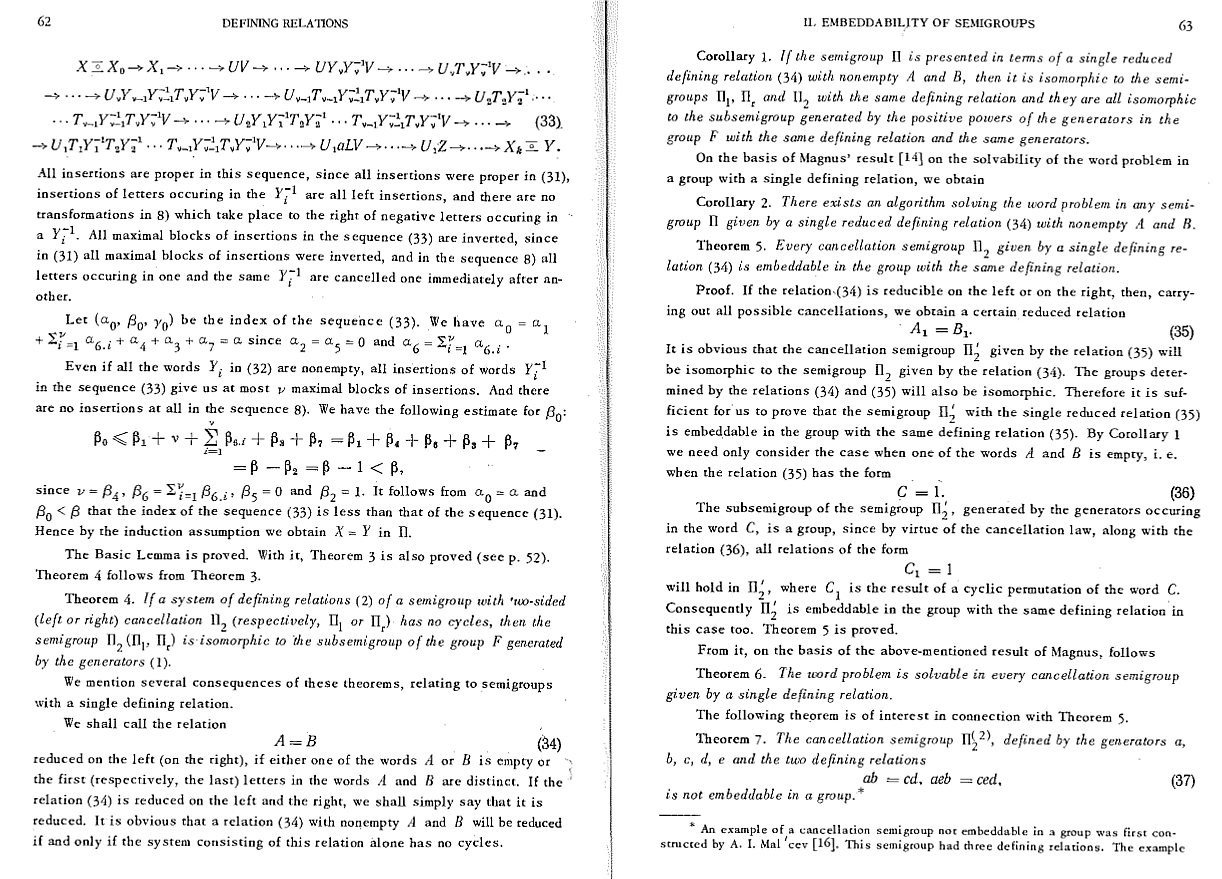
\includegraphics[height=0.65\textheight]{adjan.png}
	\end{center}

	\pause
	\vspace{-0.5cm}
	$\sim$60 pages of cases.
\end{frame}

\begin{frame}{One-relation special monoids}
	Zhang (1992) reproved the same result in 3 pages using rewriting systems. In both cases, the word problem for the semigroup is reduced to the word problem for the semigroup's group of units:\pskip

	\pause
	The \textbf{group of units} of a semigroup $S$ is the subgroup of $S$ consisting of all the invertible elements.
\end{frame}

\begin{frame}{One-relation special monoids}
	\begin{block}{Theorem (Zhang)}
		In a monoid $M$ with a presentation of the form
			\[ \Mon \langle a_1, \ldots, a_m \mid w_1 = \epsilon, \ldots, w_n = \epsilon \rangle, \]
		there is a presentation for the group of units with $n$ relations.
	\end{block}

	\pause
	\begin{block}{Corollary}
		If $M$ is a one-relator special monoid, the word problem for the group of units is solvable.
	\end{block}

	This follows from the above theorem and Magnus' result.
\end{frame}


\begin{frame}{Inverse monoids}
	A monoid in which element has an `inverse', in a slightly weaker sense than in a group.

	\pause
	\begin{block}{Theorem (Ivanov, Margolis, Meakin; 2001)}
		If the word problem is solvable for every inverse monoid admitting a presentation
			\[ \Inv \langle a_1, \ldots, a_m \mid w = \epsilon \rangle, \]
		then it is solvable for every one-relation semigroup.
	\end{block}
\end{frame}

\begin{frame}{A connection?}
	In their 2001 paper, Ivanov, Margolis and Meakin find a generating set for the group of units of the special inverse monoid.\pskip
	
	It is effectively the same as the generating set Zhang constructs for the group of units of a one-relation special monoid.\pskip

	But Zhang gives a whole presentation. Can we use a similar approach to find the needed relations in the inverse monoid case?
\end{frame}

\end{document}
